\documentclass[12pt, a4paper]{article}
\usepackage[utf8]{inputenc}
\usepackage{ragged2e}

\usepackage{graphicx, geometry, hyperref, wrapfig}
\usepackage[dvipsnames]{xcolor}

\definecolor{silver}{RGB}{200,200,200}
\hypersetup{colorlinks=true, linkcolor=RoyalBlue, urlcolor=RoyalBlue}

 \geometry{
 a4paper,
 total={175mm,257mm},
 left=20mm,
 top=15mm,
 }

\usepackage{xcolor} % for defining colour
\usepackage{titlesec} % for customizing sections

% \usepackage{times}        % Use Times New Roman font
% \usepackage{helvet}       % Use Helvetica font
\usepackage{palatino}

\usepackage[T1]{fontenc}

\setlength\parindent{0pt}

% %%%%%%%%%%%%%%%%%%%%%%%%%%%%%%%%%%%%%%%%%%%%%%%%%%%%%%%%%%%%%%
\titleformat{\section}
{\color{UM_DarkBlue}\normalfont\large\bfseries}
{\color{UM_DarkBlue}\thesection}{1em}{}

%%%%%%%%%%%%%%%%%%%%%%%%%%%%%%%%%%%%%%%%%%%%%%%%%%%%%%%%%%%%%%%
\definecolor{UM_Brown}{HTML}{3D190D}
\definecolor{UM_DarkBlue}{HTML}{2264B0}
\definecolor{UM_LightBlue}{HTML}{1CA9E1}
\definecolor{UM_Orange}{HTML}{fEB415}

%%%%%%%%%%%%%%%%%%%%%%%%%%%%%%%%%%%%%%%%%%%%%%%%%%%%%%%%%%%%%%%%

\newcommand{\eg}{{\it e.g.}}
\newcommand{\ie}{{\it i.e.}}

% %%%%%%%%%%%%%%%%%%%%%%%%%%%%%%%%%%%%%%%%%%%%%%%%%%%%%%%%%%%%%%
% \hypersetup{
%     draft=false,
%     final=true,
%     colorlinks=true,
%     citecolor=UM_DarkBlue,
%     anchorcolor=yellow,
%     linkcolor=UM_DarkBlue,
%     urlcolor=UM_DarkBlue,
%     filecolor=green,      
%     pdfpagemode=FullScreen,
%     bookmarksopen=false
%     }
\usepackage{amsmath,amsfonts,amssymb,bm}

%%%%%%%%%%%%%%%%%%%%%%%%%%%%%%%%%%%%%%%%%%%%%%%%%%%%%%%%%%%%%
% Sets and Notations
\newcommand{\reals}{\mathbb{R}}
\newcommand{\integers}{\mathbb{Z}}

%%%%%%%%%%%%%%%%%%%%%%%%%%%%%%%%%%%%%%%%%%%%%%%%%%%%%%%%%%%%%
% Vectors and Matrices
% \renewcommand{\vec}[1]{\bm{\mathrm{#1}}}
\newcommand{\dotp}{\,\boldsymbol{\cdot}\,}
\newcommand{\grad}[1]{\vec{\nabla}#1}
\renewcommand{\div}[1]{\vec{\nabla}\!\dotp\!\vec{#1}}
\newcommand{\curl}[1]{\vec{\nabla}\!\times\!\vec{#1}}



%%%%%%%%%%%%%%%%%%%%%%%%%%%%%%%%%%%%%%%%%%%%%%%%%%%%%%%%%%%%%
% Derivatives
\newcommand{\dv}[2]{\frac{d#1}{d#2}}
\newcommand{\ndv}[3][2]{\frac{d^{\,#1}#2}{d#3^{\,#1}}}

\newcommand{\pdv}[2]{\frac{\partial#1}{\partial#2}}
\newcommand{\npdv}[3][2]{\frac{\partial^{\,#1}#2}{\partial#3^{#1}}}
 
\title{OWO-GAship}
\author{Anik Mandal}
\date{January 2025}
\pagenumbering{arabic}

%====================================================================================================
\begin{document}

\begin{minipage}[t][][c]{0.1\textwidth}
    \begin{flushleft}
        
\includegraphics[height=2.5cm]{tex-resources/Ashoka Logo.png}
    \end{flushleft}
\end{minipage}
\begin{minipage}[t][][c]{0.85\textwidth}
    \begin{center}
        {\LARGE Oscillations, Wave and Optics}\\ \vspace{0.5em}
        \textsc{(Spring 2025)}\\
        \vspace{1em}
        \textbf{\Large ASSIGNMENT-5} \\
    \end{center}
\end{minipage}
\vspace{10pt}\\
\rule[0em]{\textwidth}{0.75pt}

\flushleft{Topics: Travellling Waves}\hfill 
Total Marks: 40   \\
\flushleft{Date: 24th Mar, 2025}\hfill
\fbox{\textbf{\large 
Due: 6th Apr, 2025} (EoD)}\\
\vspace{.2cm}
\rule[0em]{\textwidth}{1.75pt}
\vspace{-1cm}
%====================================================================================================
%====================================================================================================
\justifying

\section*{Problem-1 \hfill \textbf{[10]}}
Consider a junction of three co-axial transmission lines of impedances $Z_1$, $Z_2$, and $Z_3$ whose 
inner and outer conductors are connected as shown in Figure-\ref{fig:Transmission_line}. Suppose that 
a signal is incident on the junction along the line whose impedance is $Z_1$.

\begin{figure}[h]
    \centering
    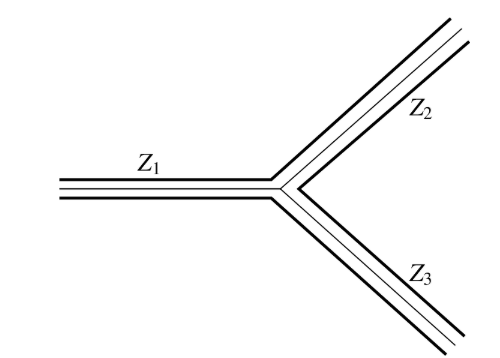
\includegraphics[scale=0.4]{figs/Transmission_lines.png}
    \caption{}
    \label{fig:Transmission_line}
\end{figure}

\textbf{(i)} Show that the coefficient of reflection is
\begin{align*}
    R = \left[\frac{Z_2 Z_3-Z_1 (Z_2+Z_3)}{Z_2 Z_3+Z_1 (Z_2+Z_3)}\right]^{2},
\end{align*}
and that the fractions of the incident power that are transmitted down the lines with impedances 
$Z_2$ and $Z_3$ are
\begin{align*}
    T_2= \frac{4 Z_1 Z_2 Z_3^{2}}{[Z_2 Z_3+Z_1 (Z_2+Z_3)]^{2}}\\	   
    T_3= \frac{4 Z_1 Z_2^{ 2} Z_3}{[Z_2 Z_3+Z_1 (Z_2+Z_3)]^{2}}	   
\end{align*}
respectively.

\textbf{(ii)} Hence, deduce that if the lines all have the same impedance then $R=1/9$ and 
$T_2=T_3=4/9$.

\textbf{(iii)} Demonstrate, further, that if
\begin{align*}
    \frac{1}{Z_1}=\frac{1}{Z_2}+\frac{1}{Z_3}
\end{align*}
then there is no reflection, and
\begin{align*}
    \frac{T_2}{T_3} = \frac{Z_3}{Z_2}
\end{align*}
This analysis suggests how one might construct a non-reflecting junction between three transmission 
lines that diverts a given fraction of the incident power into one of the outgoing lines, and the 
remainder of the power into the other outgoing line. \hfill\textbf{6+2+2}

\section*{Problem-2 \hfill \textbf{[5]}}
Consider the problem investigated in the previous question. Suppose that
\begin{align*}
    \frac{1}{Z_1}=\frac{1}{Z_2}+\frac{1}{Z_3}
\end{align*}
which implies that there is no reflection when a signal is incident on the junction along the 
transmission line whose impedance is $Z_1$. Suppose, however, that the signal is incident along 
the transmission line whose impedance is $Z_2$.

\textbf{(i)} Show that, in this case, the coefficient of reflection is
\begin{align*}
    R=\left(\frac{Z_2}{Z_2+Z_3}\right)^{2}
\end{align*}

\textbf{(ii)} Likewise, show that the coefficient of reflection is
\begin{align*}
    R=\left(\frac{Z_3}{Z_2+Z_3}\right)^{2}
\end{align*}
if the signal is incident along the transmission line whose coefficient of reflection is $Z_3$.
This analysis indicates that the lossless junction considered in the previous question can only 
be made non-reflecting when the signal is incident along one particular transmission line.
\hfill\textbf{3+2}

\section*{Problem-3 \hfill \textbf{[5]}}
Sound waves travel horizontally from a source to a receiver. Let the source have the speed $u$, and 
the receiver the speed $v$ (in the same direction). In addition, suppose that a wind of speed $w$ 
(in the same direction) is blowing from the source to the receiver. Show that if the source emits 
sound whose frequency is $f_0$ in still air then the frequency recorded by the receiver is
\begin{align*}
    f =\left(\frac{V-v+w}{V-u+w}\right)f_0
\end{align*}
where $V$ is the speed of sound in still air. Note that if the velocities of the source and receiver 
are the same then the wind makes no difference to the frequency of the recorded signal.

\section*{Problem-4 \hfill \textbf{[10]}}
In quantum mechanical formalism, we solve Schrodinger equation (let's say our ODE) to find wave 
function of a quantum particle. Time independent form of Schrodiner equaion is given by,
\begin{align*}
    &H\psi(x) = E\psi(x)\\
    &H= -\frac{\hbar^2}{2m}\frac{\partial^2}{\partial x^2} + V(x)
\end{align*}
where H is the Hamiltonian operator and V(x) is the potential felt by the particle.
Consider a negative delta potential of form $V(x) = -\alpha\delta(x)$ ($\alpha$ is some scale factor),
and also consider energy of the particle to be positive that is $E>0$ and 
$k^2 = \frac{-2mE}{\hbar^2} <0$. 

\textbf{(i)} Now solve the time independent Schrodiner equation in regions (i) $x<0$ and (ii) $x>0$ 
seperately and get the general solutions. (Take the general soution in complex form $\exp(\pm ikx)$, to ease our task!) 

\textbf{(ii)} A valid wave function demands 
\begin{itemize}
    \item The wavefunction to be continuous everywhere.
    \item Its first derivative $\frac{\partial \psi}{\partial x}$ is also continuous unless an 
    infinite potential is present. In that case wave function will go to zero at that point and first
    derivative can have finite discontinuity.
\end{itemize}
Use the first condition to get a relation between coefficients in the general soltions in both regions.

\textbf{(iii)} If you integrate the Schrodiner equaion in limit $-\epsilon$ to $\epsilon$ for 
$\epsilon \rightarrow 0$ you should get a relation,
\begin{align*}
    \Delta(\frac{\partial \psi}{\partial x}) = \frac{\partial \psi}{\partial x}|_+ - \frac{\partial \psi}{\partial x}|_- 
    = -\frac{2m\alpha}{\hbar^2}\psi(x=0)
\end{align*}
Try yourself and use the derived relation to find another relation between the coefficients of the 
general solutions.

\textbf{(iv)} In the general solutions define each components and their direction of propagation. Now,
suppose a wave is comming from $-\infty$ and moving along positive x-direction, after encountering the 
potential some fraction of the wave will get through the potential and keep travelling along positive 
x-direction and rest will get reflected back towards $-\infty$ (You should ignore the component of the 
general soltion that describes wave propagation along negative x-direction in $x>0$ region as that is 
irrelevent for this given problem). Using the two relations we have derived earlier, try to find 
analytical form of reflection and transmission coefficients (Reflection coefficient is the square of 
the ratio of the reflected wave amplitude and incident wave amplitude. And transmission coefficient is 
the square of the ratio of the transmitted wave amplitude and incident wave amplitude).

\textbf{(v)} Try to plot the the reflection and transmission coefficient as a function of particle 
energy in the same graph. (You can use any graphing calculators/programming language for plotting) \\
And derive the condition for which both the coefficients will be same.
\hfill\textbf{2 + 1 + 2 + 3 + 2}

\section*{Problem-4 \hfill \textbf{[10]}}
For a step potential of form,
\begin{align*}
    V(x) = \begin{cases}
        0, & x < 0 \\
        V_0, & 0 \leq x \leq a\\
        0, & x > a
\end{cases}
\end{align*}
Similar to previous treatment,  we can get wave functions of the particle comming from $-\infty$ 
in these three regions as,
\begin{align*}
    \psi(x) = \begin{cases}
        \psi_1 = A\exp(ik_1x) + B\exp(-ik_1x), & x < 0 \\
        \psi_2 = C\exp(ik_2x) + D\exp(-ik_2x), & 0 \leq x \leq a\\
        \psi_3 = E\exp(ik_1x), & x > a
\end{cases}
\end{align*}
Where $k_1 = \sqrt{2mE}/\hbar^2$, and $k_2 = \sqrt{2m(E-V_0)}/\hbar^2$.

\textbf{(i)} Use the conditions for a valid wavefunction at two boundaries (x=0 and x=a) to derive a set 
of relations between coefficients. 

\textbf{(ii)} Derive the analytical form of reflection and transmission coefficient.

\textbf{(iii)} Plot the coefficients as a function of energy.(You can use any graphing calculators/
programming language for plotting)\\
Check what happens to transmission coefficient when $E < V_0$, and descibe the result.
\hfill\textbf{4 + 4 + 2}
\end{document}
